%%%%%%%%%%%%%%%%%%%%%%%%%%%%%%%%% COMMENT THIS TO COMPILE main.tex %%%%%%%%%%%%%%%%%%%%%%%%%%%%%%%%
%\documentclass[a4paper,12pt]{report}
\usepackage[english]{babel}
\usepackage[left=2cm,right=2cm,top=2cm,bottom=2cm]{geometry}
%\usepackage{mathtools}
\usepackage{amsthm}     % for definitions and theorems
\usepackage[many]{tcolorbox}    % boxes around definitions and theorems
%\usepackage{amsmath}
%\usepackage{nccmath}
\usepackage{amssymb}    % \ltimes
\usepackage{etoolbox}   % for start of Chapter
%\usepackage{amsfonts}
\usepackage{physics}    % for all Physics related
\usepackage{dsfont}     % for the identity matrix symbol \1
%\usepackage{mathrsfs}

\usepackage{titling}
\usepackage{indentfirst}

\usepackage{bm}
\usepackage[dvipsnames]{xcolor}
\usepackage{cancel}

\usepackage{xurl}
\usepackage[colorlinks=true]{hyperref}

\usepackage{float}
\usepackage{graphicx}
\usepackage{subcaption}
%\usepackage{tikz}

\usepackage{ctable}     % tabelas
\renewcommand{\P}{\phantom{+}}  % empty space to indent things
\usepackage{multirow}
\usepackage{tabulary}

%%%%%%%%%%%%%%%%%%%%%%%%%%%%%%%%%%%%%%%%%%%%%%%%%%%

\newcommand{\eps}{\epsilon}
\newcommand{\vphi}{\varphi}
\newcommand{\cte}{\text{cte}}

\newcommand{\N}{{\mathbb{N}}}
\newcommand{\Z}{{\mathbb{Z}}}
%\newcommand{\Q}{{\mathbb{Q}}}
\newcommand{\C}{{\mathbb{C}}}
\renewcommand{\S}{{\hat{S}}}
%\renewcommand{\H}{\s{H}}

\renewcommand{\a}{{\vb{a}}}
\renewcommand{\b}{{\vb{b}}}
\renewcommand{\d}{{\dagger}}
\newcommand{\up}{{\uparrow}}
\newcommand{\down}{{\downarrow}}
\newcommand{\hc}{{\text{h.c.}}}

\newcommand{\ihat}{\bm{\hat{\imath}}}
\newcommand{\jhat}{\bm{\hat{\jmath}}}
\newcommand{\khat}{\bm{\hat{k}}}

\newcommand{\0}{{\vb{0}}}
\newcommand{\1}{\mathds{1}}
\newcommand{\E}{{\vb{E}}}
\newcommand{\B}{{\vb{B}}}
\renewcommand{\u}{{\vb{u}}}
\renewcommand{\v}{{\vb{v}}}
\renewcommand{\r}{{\vb{r}}}
\newcommand{\R}{{\vb{R}}}
\newcommand{\Q}{{\vb{Q}}}
\newcommand{\G}{{\vb{G}}}
\newcommand{\g}{{\vb{g}}}
\renewcommand{\k}{{\vb{k}}}
\newcommand{\K}{{\vb{K}}}
\newcommand{\p}{{\vb{p}}}
\newcommand{\q}{{\vb{q}}}
\newcommand{\F}{{\vb{F}}}
\renewcommand{\t}{{\vb{t}}}
\newcommand{\vtau}{{\bm{\tau}}}
\newcommand{\vdelta}{{\bm{\delta}}}

% COLORED SYMMETRY ELEMENTS
\newcommand{\Ct}{{\textcolor{Cyan}{C_3}}}
\newcommand{\Ctn}[1]{{\textcolor{Cyan}{C_3^{\textcolor{black}{#1}}}}}
\newcommand{\Cs}{{\textcolor{ForestGreen}{C_6}}}
\newcommand{\Csn}[1]{{\textcolor{ForestGreen}{C_6^{\textcolor{black}{#1}}}}}
\newcommand{\sd}{{\textcolor{RoyalBlue}{\sigma_d}}}
\newcommand{\sdn}[1]{{\textcolor{RoyalBlue}{\sigma_d^{\textcolor{black}{#1}}}}}
\newcommand{\sdp}{{\textcolor{RoyalBlue}{\sigma_d'}}}
\newcommand{\sdpp}{{\textcolor{RoyalBlue}{\sigma_d''}}}
\newcommand{\sv}{{\textcolor{Orange}{\sigma_v}}}
\newcommand{\svn}[1]{{\textcolor{Orange}{\sigma_v^{\textcolor{black}{#1}}}}}
\newcommand{\svp}{{\textcolor{Orange}{\sigma_v'}}}
\newcommand{\svpp}{{\textcolor{Orange}{\sigma_v''}}}

\newcommand{\s}{\sigma}
%\newcommand{\prodint}[2]{\left\langle #1 , #2 \right\rangle}
\newcommand{\cc}[1]{\overline{#1}}
\newcommand{\Eval}[3]{\eval{\left( #1 \right)}_{#2}^{#3}}
\newcommand{\sg}[2]{\{ #1 \mid #2 \}}

\newcommand{\unit}[1]{\; \mathrm{#1}}

\newcommand{\n}{\medskip}
\newcommand{\e}{\quad \mathrm{and} \quad}
\newcommand{\ou}{\quad \mathrm{or} \quad}
\newcommand{\virg}{\, , \;}
\newcommand{\ptodo}{\forall \,}
\renewcommand{\implies}{\; \Rightarrow \;}
%\newcommand{\eqname}[1]{\tag*{#1}} % Tag equation with name

\setlength{\droptitle}{-7em}

\makeatletter
\patchcmd{\chapter}{\if@openright\cleardoublepage\else\clearpage\fi}{}{}{}  % start 'Chapter' at the same page. needs package etoolbox
\makeatother

%% Theorems, definitions, proofs
\theoremstyle{definition}

\newtheorem{definition}{Definition}[section]
\tcolorboxenvironment{definition}{
  colback=blue!5!white,
  boxrule=0pt,
  boxsep=1pt,
  left=2pt,right=2pt,top=2pt,bottom=2pt,
  oversize=2pt,
  sharp corners,
  before skip=\topsep,
  after skip=\topsep,
}

\newtheorem{theorem}{Theorem}[section]
\tcolorboxenvironment{theorem}{
  colback=blue!5!white,
  boxrule=0pt,
  boxsep=1pt,
  left=2pt,right=2pt,top=2pt,bottom=2pt,
  oversize=2pt,
  sharp corners,
  before skip=\topsep,
  after skip=\topsep,
}

%\begin{document}
%%%%%%%%%%%%%%%%%%%%%%%%%%%%%%%%% COMMENT THIS TO COMPILE main.tex %%%%%%%%%%%%%%%%%%%%%%%%%%%%%%%%


%%%%%%%%%%%%%%%%%%%%%%%%%%%%%%%%%%%%%%%%%%%%%%%%%%%%%%%%%%%%%%%%%%%%%%%%%%%%%%%%%%%%%%%%%%%%%%%%%%
\chapter{Introduction} \label{ch:intro}
%%%%%%%%%%%%%%%%%%%%%%%%%%%%%%%%%%%%%%%%%%%%%%%%%%%%%%%%%%%%%%%%%%%%%%%%%%%%%%%%%%%%%%%%%%%%%%%%%%

Carbon is undoubtedly one of the most essential elements for the formation of life, largely due to its remarkable versatility in bonding, which enables the formation of a vast array of complex compounds. Among materials composed solely of carbon atoms, graphite is one of which we are very familiar since elementary school, as it used in pencils for drawing. Graphite is an allotrope of carbon, consisting of multiple layers stacked together and held by weak van der Waals forces. When writing with a pencil, some graphite layers transfer onto the paper, allowing for drawing and writing.

In 2004, Andre Geim, Konstantin Novoselov, et. al. \cite{novoselov_2004} successfully isolated a single sheet of graphite using the ``sticky tape method'', allowing them to study its properties. This single atomic layer, known as graphene, was the first two-dimensional (2D) material ever discovered. Graphene exhibits extraordinary properties, including exceptional electrical conductivity, mechanical strength, flexibility, transparency, and thermal conductivity. Its unique combination of properties makes it a promising candidate for a wide range of applications, from electronics and energy storage to composite materials and biomedical devices. The discovery and stabilization of graphene marked a breakthrough, inaugurating the field of 2D materials and earning Geim and Novoselov the Nobel Prize in Physics in 2010. Since then, the family of 2D materials has expanded to include metals like NbSe\(_2\), semiconductors such as transition metal dichalcogenides (TMDs), and insulators like hexagonal boron nitride (hBN). Notably, hBN is the primary substrate for graphene due to its wide bandgap ($\sim 6 \unit{eV}$), chemical inertness, and favorable dielectric properties. Encapsulating graphene in hBN shields it from environmental contaminants and significantly enhances its electronic transport properties.

These 2D materials can be stacked to form van der Waals heterostructures, held together by weak interlayer van der Waals forces, allowing the engineering of novel properties at their interfaces. While the behavior of single-layer materials like graphene is well understood, predicting the properties of multilayer heterostructures remains a challenge. A particularly fascinating type of heterostructure are the moiré materials, created by stacking two layers with a slight twist angle or mismatched lattice constants. This misalignment generates a moiré pattern, where the local atomic arrangement varies periodically over a much larger scale than the unit cell of each layer. The moiré pattern acts as a long-wavelength potential, dramatically altering the electronic and structural properties of the system. These emergent states differ fundamentally from those of the individual layers, giving rise to entirely new physical behaviors.

The ability to control the twist angle introduces a new degree of freedom, giving rise to the field of \textit{twistronics}. A landmark moment in this field came in 2018 with two papers published by Jarillo-Herrero and colleagues \cite{cao2018, cao2018_correlated}. These works reported the discovery of correlated insulating and superconducting states in ``magic angle'' twisted bilayer graphene (MATBG), sparking intense theoretical interest and accelerating research into the properties of graphene-based systems.
%\textbf{MAIS TEXTO AQUI. FALAR DA WANNIER OBSTRUCTION E PORQUE É NECESSÁRIO O THF model}.
This thesis focuses on MATBG, where we will investigate its symmetry and topological characteristics, aiming to provide an understanding of the fundamental principles underlying the Topological Heavy Fermion model \cite{topoheavyfermion2022}.

\pagebreak

This chapter serves as an introduction to the complexities and intriguing properties of twisted bilayer graphene (TBG). Section \ref{sec:monolayer_graphene} begins with a brief discussion of the tight-binding model for monolayer graphene, laying the groundwork and terminology essential for later analyses. In Section \ref{sec:experimental_tbg}, we delve into key experimental findings from the literature that highlight the remarkable characteristics of TBG. Finally, Section \ref{sec:outline_thesis} outlines the structure of this thesis, detailing the approach and organization of the subsequent chapters as they tackle the central challenges of the subject.

%%%%%%%%%%%%%%%%%%%%%%%%%%%%%%%%%%%%%%%%%%%%%%%%%%%%%%%%%%%%%%%%%%%%%%%%%%%%%%%%%%%%%%%%%%%%%%%%%%
\section{Monolayer Graphene} \label{sec:monolayer_graphene}
%%%%%%%%%%%%%%%%%%%%%%%%%%%%%%%%%%%%%%%%%%%%%%%%%%%%%%%%%%%%%%%%%%%%%%%%%%%%%%%%%%%%%%%%%%%%%%%%%%

To establish consistent terminology and notation, we will begin by outlining a tight-binding model for monolayer graphene, which will serve as the foundation for much of our analysis. The models for twisted bilayer graphene are also strongly influenced by this approach. Graphene is an allotrope of graphite and consists of a honeycomb lattice of carbon atoms. These atoms are bonded via $sp^2$ hybridization, with an average interatomic distance of \( d = 1.42 \, \AA \). In this structure, three valence electrons from each carbon atom form $\sigma$ bonds, while the remaining valence electron resides in a $p_z$ orbital, which plays a dominant role in the material's electronic properties. A schematic of the lattice is shown in Figure \ref{fig:graphene-lattice_a}.

%Our convention is zig-zag in horizontal direction and arm-chair in vertical direction.

\begin{figure}[H]
\centering
\begin{subfigure}{.48\textwidth}
  \centering
  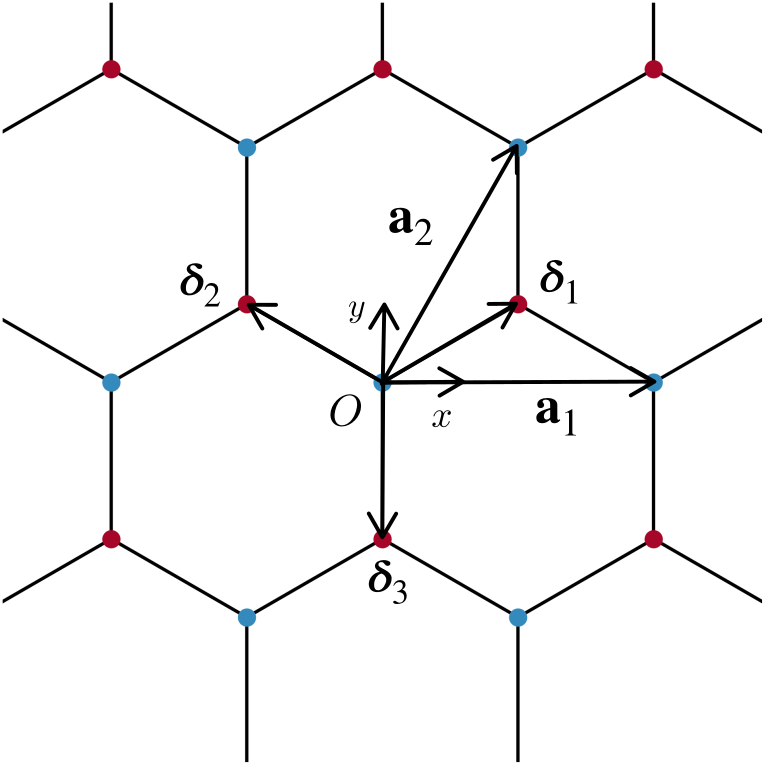
\includegraphics[height=.78\linewidth]{fig/honeycomb_coordinates_deltas.png}
  \caption{Graphene's lattice with atoms labeled $\textcolor{blue}{A}$ (blue) and $\textcolor{red}{B}$ (red), both being identical carbon atoms.}
  \label{fig:graphene-lattice_a}
\end{subfigure} \hfill
\begin{subfigure}{.48\textwidth}
  \centering
  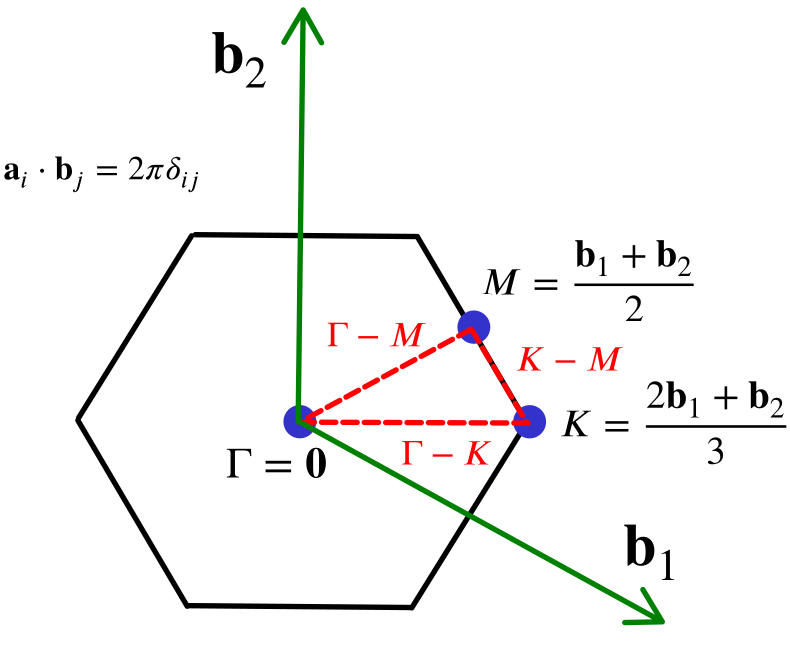
\includegraphics[height=.78\linewidth]{fig/honeycomb_tqc_BZ.png}
  \caption{Graphene Brillouin Zone with high-symmetry momentum points labeled as $\Gamma$, $K$, and $M$.}
  \label{fig:graphene-lattice_b}
\end{subfigure}
%\caption{}
\label{fig:graphene-lattice}
\end{figure}

The lattice vectors are defined as \(\vb{a}_1 = a \qty(1, 0)\) and \(\vb{a}_2 = a \qty(\frac{1}{2}, \frac{\sqrt{3}}{2})\), with $a = d\sqrt{3} = 2.46 \, \AA$. The unit cell area is given by \( A_1 = \abs{\a_1 \times \a_2} = \frac{\sqrt{3}}{2} a^2 \). The momentum lattice vectors \(\b_1\) and \(\b_2\) satisfy the relation \(\a_i \vdot \b_j = 2\pi \delta_{ij}\) and can be derived as follows:
\begin{equation} \label{eq:monolayer-bvecs}
\b_1 = \frac{2\pi}{A_1} \a_2 \times \a_3 = \frac{4\pi}{\sqrt{3} a } \qty(\frac{\sqrt{3}}{2}, -\frac{1}{2}), \quad
\b_2 = \frac{2\pi}{A_1} \a_3 \times \a_1 = \frac{4\pi}{\sqrt{3} a } \qty(0, 1),
\end{equation}
where for calculation purposes, we used \(\a_3 = \vu{z}\).

The two main Dirac points lie at the edge of the Brillouin Zone (BZ), as illustrated in Figure \ref{fig:graphene-lattice_b}, and are defined as:
\begin{equation} \label{eq:monolayer-dirac-points}
K = \frac{2\b_1 + \b_2}{3} = \frac{4\pi}{3a} (1, 0) , \quad K' = -K.
\end{equation}

Ignoring the spin degree of freedom (since spin-orbit coupling is weak in graphene and magnetic fields are not considered), the tight-binding Hamiltonian with only nearest-neighbor hoppings is expressed as:
\begin{equation} \label{eq:monolayer-tight-binding}
H = -t \sum_{\R} c^\d_A(\R) \qty(c_B(\R + \vdelta_1) + c_B(\R+\vdelta_2) + c_B(\R+\vdelta_3)) + \hc,
\end{equation}
where $t = 2.97 \unit{eV}$ according to \textit{ab initio} calculations \cite{handbook2019}, and \(\R = n_1 \a_1 + n_2 \a_2\), with integers \(n_1, n_2\), runs over all the lattice sites of the underlying Bravais triangular lattice. Applying the following Fourier transformation:
\begin{equation} \label{eq:monolayer-fourier}
c_{\alpha}^\d(\r) = \frac{1}{\sqrt{N}} \sum_{\k \in \text{BZ}} e^{-i \k \vdot \r} c_\alpha^\d(\k),
\end{equation}
we obtain the Hamiltonian in momentum space
\begin{equation} \label{eq:monolayer-tight-binding2}
H = \sum_{\k}
\begin{pmatrix}
c_A^\d(\k) & c_B^\d(\k)
\end{pmatrix}
H_\k
\begin{pmatrix}
c_A^\d(\k) \\ c_B^\d(\k)
\end{pmatrix},
\end{equation}
where the matrix \(H_\k\) is
\begin{equation} \label{eq:hamiltonian_k_monolayer}
H_\k =
\begin{pmatrix}
0 & -t f(\k) \\
-t f^{\dagger}(\k) & 0
\end{pmatrix},
\end{equation}
and the function \(f(\k)\) is given by
\begin{equation} \label{eq:monolayer-fk}
f(\k) = e^{i \k \vdot \bm{\delta}_1} + e^{i \k \vdot \bm{\delta}_2} + e^{i \k \vdot \bm{\delta}_3} =
e^{-idk_y} + 2 e^{\frac{idk_y}{2}} \cos(\frac{\sqrt{3}}{2} dk_x),
\end{equation}
where \(\bm{\delta}_1 = \frac{\a_1 + \a_2}{3} = d \qty(\frac{\sqrt{3}}{2}, \frac{1}{2})\), \(\bm{\delta}_2 = \frac{-2 \a_1 + \a_2}{3} = d \qty(-\frac{\sqrt{3}}{2}, \frac{1}{2})\), and \(\bm{\delta}_3 = \frac{\a_1 - 2 \a_2}{3} = d \qty(0, -1)\) are the vectors connecting the three nearest neighbor sites.

The eigenenergies of the Hamiltonian matrix \(H_\k\) are \(E_\pm(\k) = \pm t \abs{f(\k)}\). The Dirac points \(K\) and \(K' = -K\) correspond to the zeros of \(f(\k)\), i.e., \(f(\pm K) = 0\). In the vicinity of these points, the dispersion relation is approximately linear, as illustrated in Figure \ref{fig:monolayer_dispersion}.
\begin{equation} \label{eq:linear_Ek_monolayer}
E(\K + \q) = v_0 \abs{\q} + O\left(\frac{\abs{\q}}{\abs{K}}\right)^2,
\end{equation}
where \( v_0 = \frac{3td}{2} \) is the Fermi velocity, adopting the convention \(\hbar = 1\). The \(p_z\) electrons in graphene exhibit a dispersion relation analogous to that of relativistic Dirac particles, though their velocity, \(v_0 \approx 10^6 \, \text{m/s}\), is approximately 300 times smaller than the speed of light, \(c = 3 \times 10^8 \, \text{m/s}\).

\begin{figure}[H]
\centering
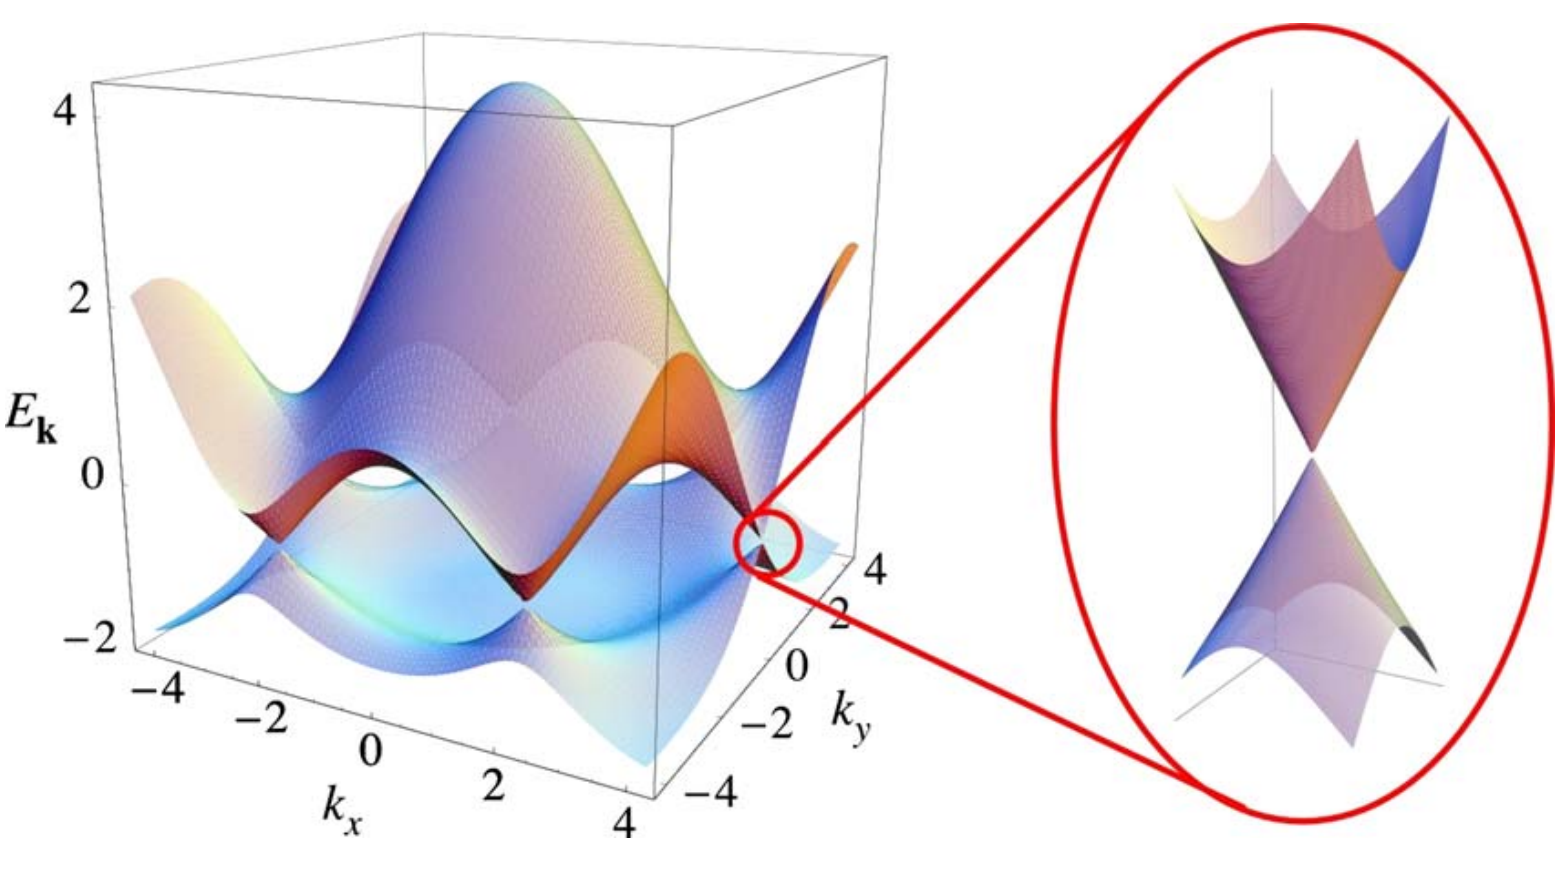
\includegraphics[width=0.8\linewidth]{fig/monolayer_dispersion.png}
\caption{Electronic band structure of graphene (energy in eV). Adapted from \cite{geim2009}.}
\label{fig:monolayer_dispersion}
\end{figure}

%%%%%%%%%%%%%%%%%%%%%%%%%%%%%%%%%%%%%%%%%%%%%%%%%%%%%%%%%%%%%%%%%%%%%%%%%%%%%%%%%%%%%%%%%%%%%%%%%%
\section{Twisted bilayer graphene} \label{sec:experimental_tbg}
%%%%%%%%%%%%%%%%%%%%%%%%%%%%%%%%%%%%%%%%%%%%%%%%%%%%%%%%%%%%%%%%%%%%%%%%%%%%%%%%%%%%%%%%%%%%%%%%%%

Twisted bilayer graphene (TBG), formed by stacking two graphene layers with a small twist angle, has become a highly researched material due to its rich and highly tunable electronic properties. The twist between the layers gives rise to a moiré pattern, as illustrated in Figure \ref{fig:moire_pattern}, which introduces a complex modulation of the interlayer interactions. This modulation significantly alters the band structure compared to that of monolayer graphene, as previously shown in Figure \ref{fig:monolayer_dispersion}.

\begin{figure}[H]
\centering
\begin{subfigure}{.37\textwidth}
  \centering
  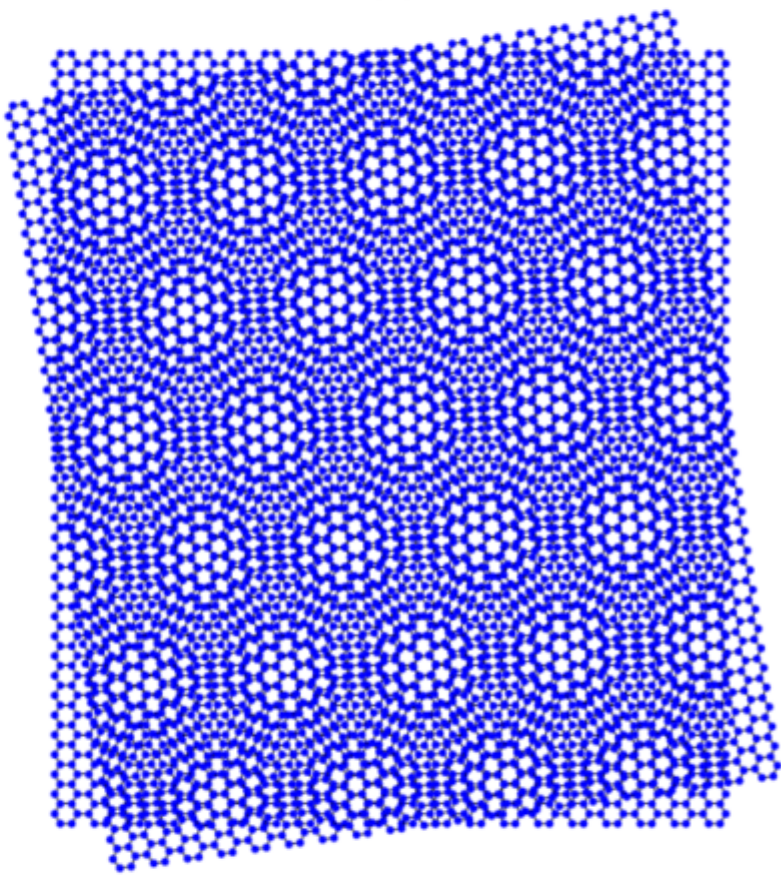
\includegraphics[height=12em]{fig/moire_pattern.png}
  \caption{Moiré pattern formed by two twisted graphene layers. Adapted from \cite{moire_pattern_figure2021}.}
  \label{fig:moire_pattern}
\end{subfigure} \hfill
\begin{subfigure}{.60\textwidth}
  \centering
  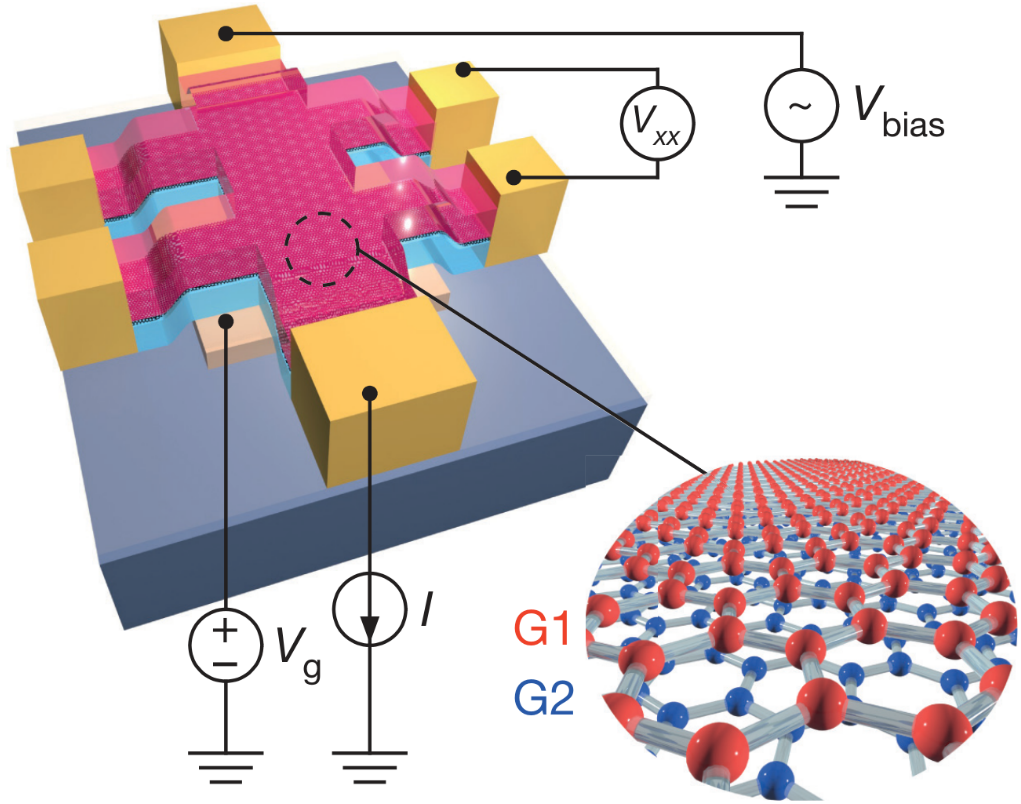
\includegraphics[height=11em]{fig/tbg_device2.png}
  \caption{Schematic of a TBG device with a four-probe setup. Hexagonal boron nitride (hBN) layers encapsulates the TBG, and a metal gate below the bottom hBN controls electron density. Adapted from \cite{cao2018}.}
  \label{fig:tbg_device2}
\end{subfigure}
\caption{Illustration of the TBG system, depicting the moiré pattern and the experimental setup.}
\label{fig:tbg_moire_device}
\end{figure}

At specific twist angles, known as \textit{magic angles}, these interactions give rise to nearly flat electronic bands near the charge neutrality point (CNP), separated from other bands by gaps on the order of tens of meV. This band flattening is a result of the interplay between intra- and interlayer hybridization energies, as shown in Figure \ref{fig:tbg_dirac_cones}. It occurs when the energy \(2w\), associated with interlayer coupling, becomes comparable to the energy difference \(\hbar v_0 k_\theta\) between the Dirac cones at the \(K^{(1)}\) and \(K^{(2)}\) points of the two layers.

\begin{figure}[H]
\centering
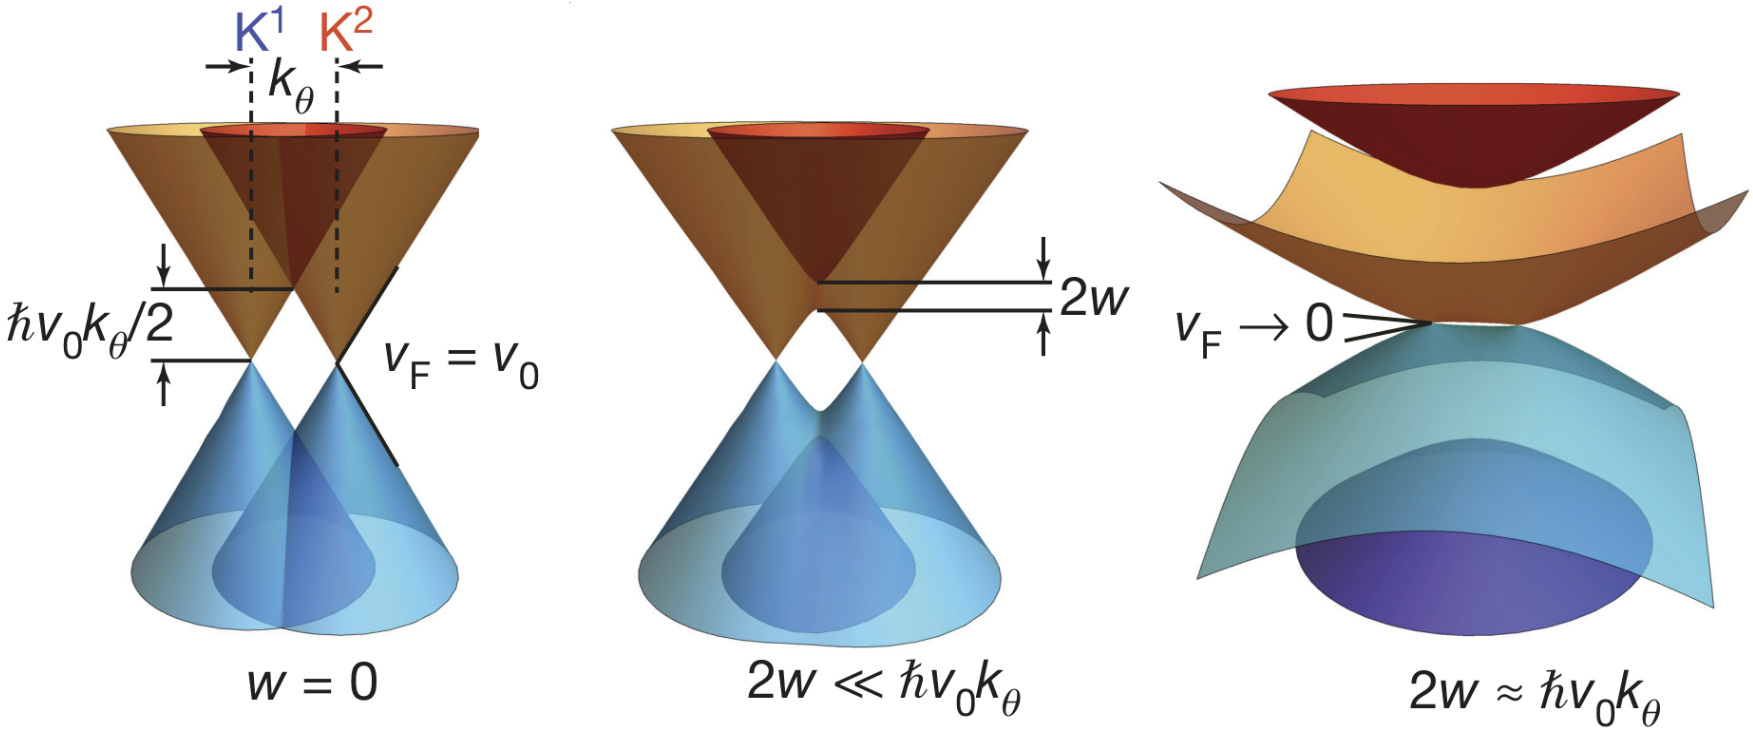
\includegraphics[width=0.70\linewidth]{fig/tbg_dirac_cones}
\caption{Illustration of interlayer hybridization in three scenarios: (1) \( w = 0 \), no interlayer coupling; (2) \( 2w \ll \hbar v_0 k_\theta \), weak interlayer coupling; and (3) \( 2w \approx \hbar v_0 k_\theta \), strong interlayer coupling. Here, \( v_0 \approx 10^6 \, \text{m/s} \) is the Fermi velocity of graphene and $k_\theta = 2 \abs{K} \sin(\theta/2)$. Adapted from \cite{cao2018_correlated}.}
\label{fig:tbg_dirac_cones}
\end{figure}

At twist angles near the magic angles, a variety of extraordinary phenomena emerge. Bistritzer and MacDonald \cite{macdonald2011} predicted that the hybridization of Dirac cones at the \(K\) and \(K'\) points leads to the opening of energy gaps at their intersections and a significant renormalization of the Fermi velocity. At the magic angles, the Fermi velocity vanishes, giving rise to isolated, narrow bands around the charge neutrality point (CNP). These near flat bands are a hallmark of twisted bilayer graphene (TBG) and have been experimentally confirmed, particularly at the first magic angle (\(\theta \approx 1.1^\circ\)), where four extremely narrow bands appear at the CNP, as illustrated in Figures \ref{fig:tbg_bandstructure_a} and \ref{fig:tbg_bandstructure_b}.

\begin{figure}[H]
\centering
\begin{subfigure}{.48\textwidth}
  \centering
  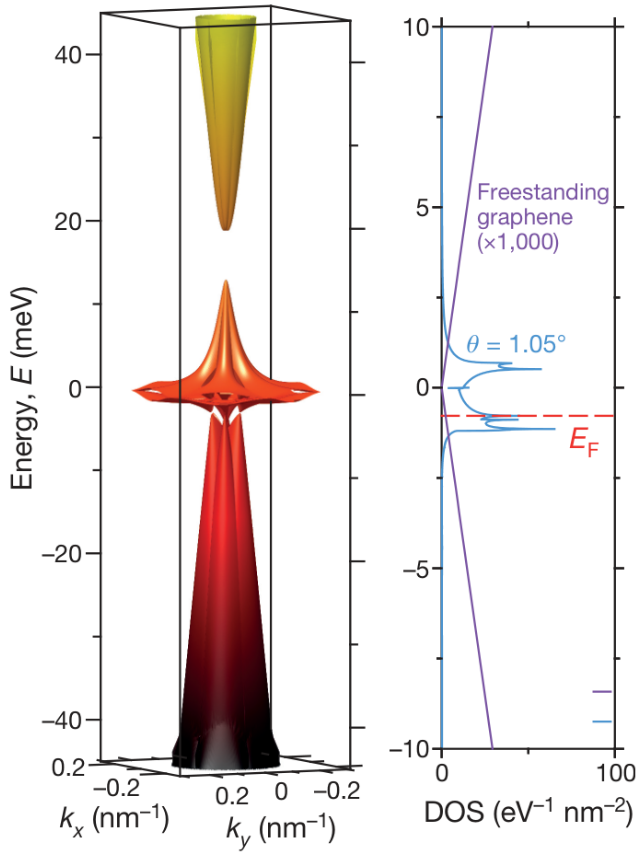
\includegraphics[height=20em]{fig/tbg_bandstructure.png}
  \caption{Band structure of TBG in \((k_x, k_y)\) momentum space within the mBZ at \(\theta = 1.05^\circ\), along with its corresponding density of states. Adapted from \cite{cao2018}.}
  \label{fig:tbg_bandstructure_a}
\end{subfigure} \hfill
\begin{subfigure}{.48\textwidth}
  \centering
  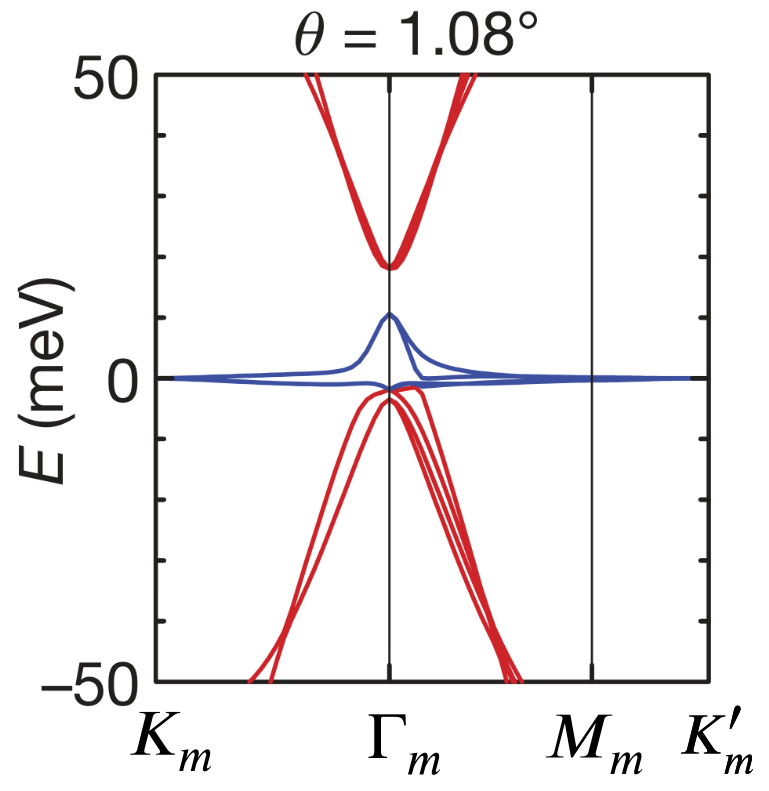
\includegraphics[height=21em]{fig/tbg_4_narrowbands.png}
  \caption{Four narrow bands at angle \(\theta = 1.08^\circ\), with the bandstructure plotted along the high-symmetry lines \(\Gamma_m - K_m - M_m - K_m'\) in the mBZ. Adapted from \cite{cao2018_correlated}.}
  \label{fig:tbg_bandstructure_b}
\end{subfigure}
\caption{Band structure of TBG in the mini Brillouin Zone (mBZ), showing the appearance of flat bands near the charge neutrality point (CNP) near the magic angle $\theta \approx 1.1^\circ$.}
\label{fig:tbg_figures_taken_from_correlated_insul}
\end{figure}


Jarillo-Herrero et al. \cite{cao2018, cao2018_correlated} discovered that doping the flat bands in TBG leads to the emergence of both insulating and superconducting phases, marking a new frontier in two-dimensional materials research. The insulating states, observed at half-fillings of the flat bands in Figure \ref{fig:tbg_conductance_filling_insulating}, are Mott insulators, driven by electron-electron interactions rather than band theory alone. These states are characterized by a sharp drop in conductance, indicating a transition from metallic to insulating behavior, with conductance exponentially suppressed below a critical temperature of approximately \(T = 4 \, \text{K}\), as shown in Figure \ref{fig:tbg_conductance_temperature_insulating}.

\begin{figure}[H]
\centering
\begin{subfigure}{.56\textwidth}
  \centering
  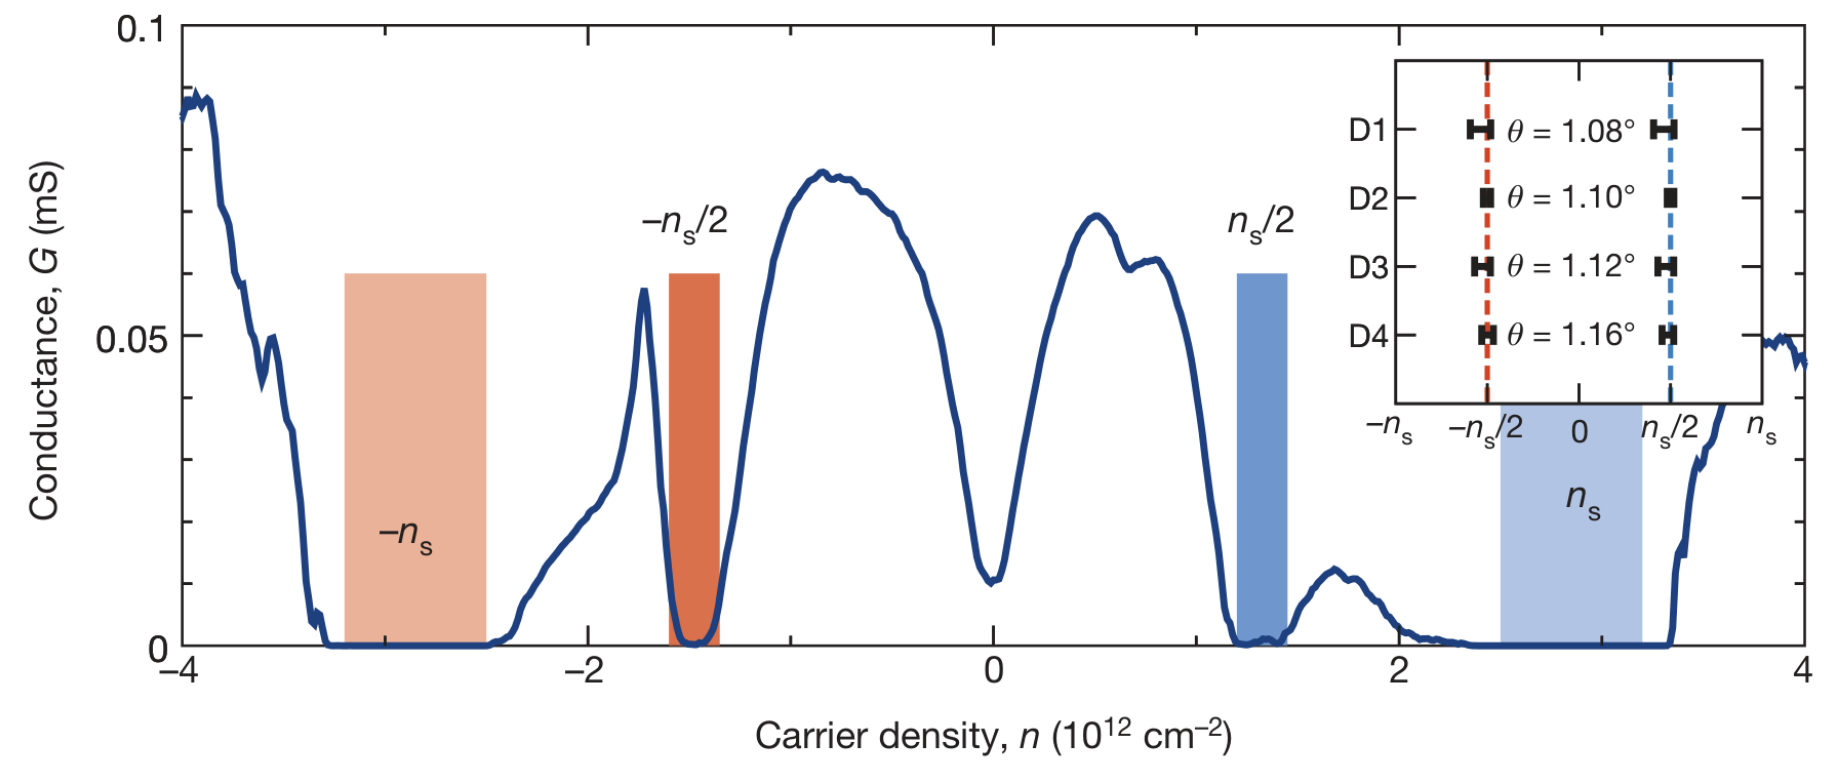
\includegraphics[height=9.5em]{fig/tbg_conductance_filling_insulating.png}
  \caption{Half-filling insulating states in MATBG. Conductance \(G\) of a TBG device with \(\theta = 1.08^\circ\) at \(T = 0.3 \, \text{K}\). Lighter-shaded regions indicate superlattice gaps at carrier density \(n = \pm n_s = \pm 2.7 \times 10^{12} \, \text{cm}^{-2}\), and darker-shaded regions show half-filling insulating states at \(n = \pm n_s/2\). Inset displays half-filling state positions across four devices.}
  \label{fig:tbg_conductance_filling_insulating}
\end{subfigure} \hfill
\begin{subfigure}{.40\textwidth}
  \centering
  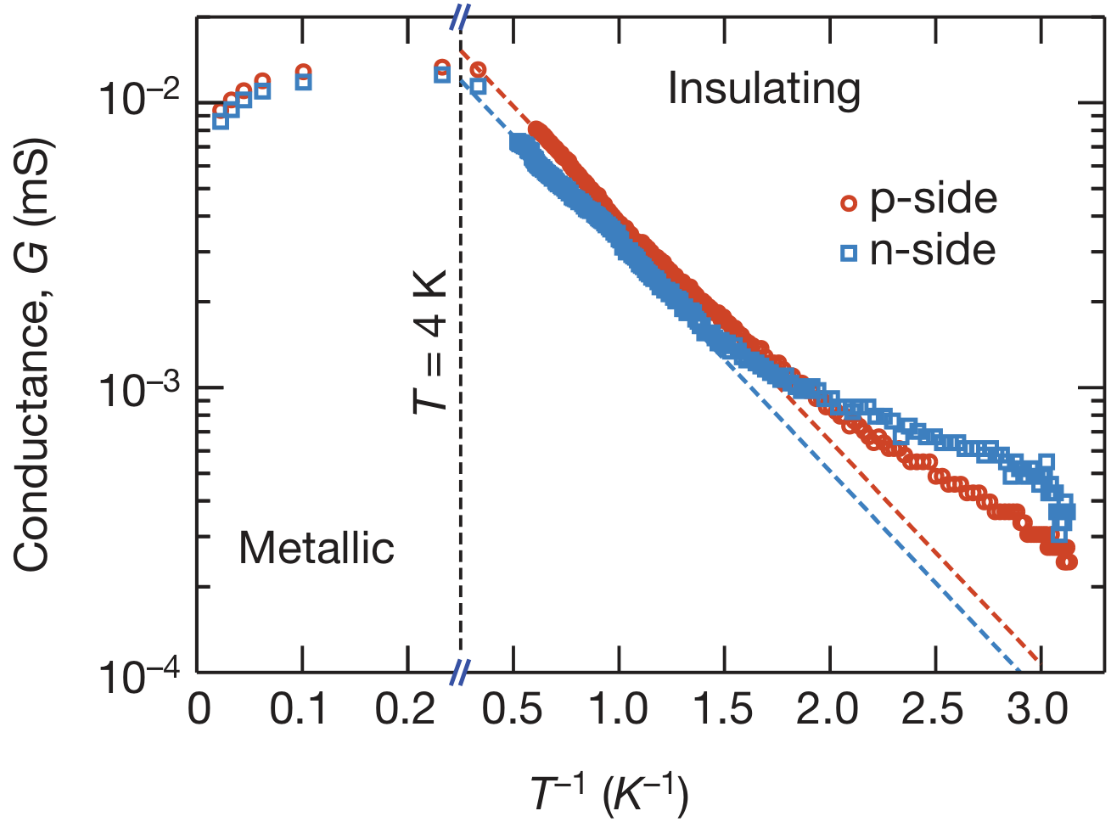
\includegraphics[height=9.5em]{fig/tbg_conductance_temperature_insulating.png}
  \caption{Minimum conductance in half-filling states at $\theta = 1.08^\circ$ for the \(p\)-side (red) and \(n\)-side (blue) of the device. The dashed lines represent exponential fits of the form \(\exp[-\Delta/(2kT)]\), with \(\Delta \approx 0.31 \, \text{meV}\) being the thermal activation gap.}
  \label{fig:tbg_conductance_temperature_insulating}
\end{subfigure}
\caption{Evidence of half-filling insulating states at the magic angle \(\theta = 1.08^\circ\). Adapted from \cite{cao2018_correlated}.}
\label{fig:tbg_insulating}
\end{figure}

When slightly doped away from the insulating states at half-filling, twisted bilayer graphene exhibits superconducting behavior, characterized by a sharp drop in resistance to zero. This superconductivity, observed at a critical temperature of \( T_c = 1.7 \, \text{K} \) for a twist angle of \( \theta = 1.05^\circ \) (Figure \ref{fig:tbg_superconductivity_b}), can be suppressed by a perpendicular magnetic field as low as \( B = 0.4 \, \text{T} \) \cite{cao2018}. The phase diagram for \( \theta = 1.16^\circ \), shown in Figure \ref{fig:tbg_superconductivity_a}, features two superconducting domes flanking the Mott insulating phase, with the system transitioning to a normal metallic state at elevated temperatures. This phase diagram shows a notable resemblance to that of high-temperature superconducting cuprates \cite{cuprate_superconductivity_lee2006}, inspiring extensive theoretical and experimental efforts to explore the origins of these phenomena.

\begin{figure}[H]
\centering
\begin{subfigure}{.48\textwidth}
  \centering
  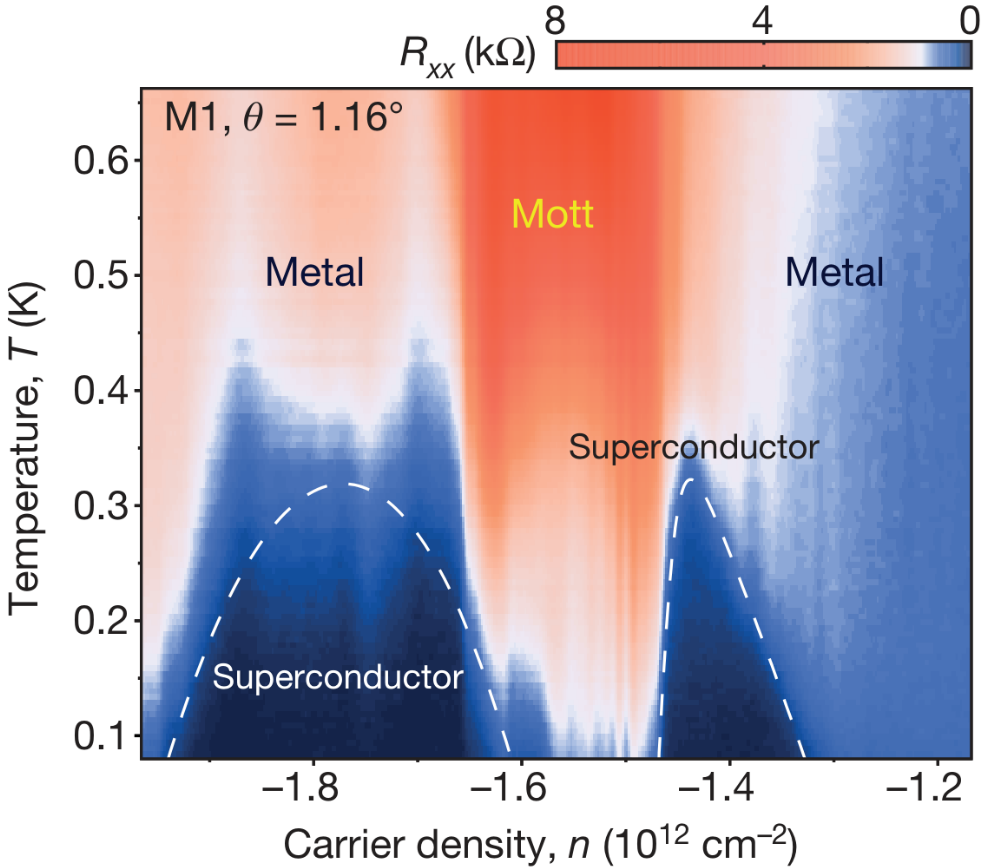
\includegraphics[height=17em]{fig/tbg_Tc_superconductivity_M1.png}
  \caption{Phase diagram for \(\theta = 1.16^\circ\) showing weak superconductivity with a critical temperature \(T_c = 0.5 \, \text{K}\). The phase diagram resembles that of cuprates \cite{cuprate_superconductivity_lee2006}.}
  \label{fig:tbg_superconductivity_a}
\end{subfigure} \hfill
\begin{subfigure}{.48\textwidth}
  \centering
  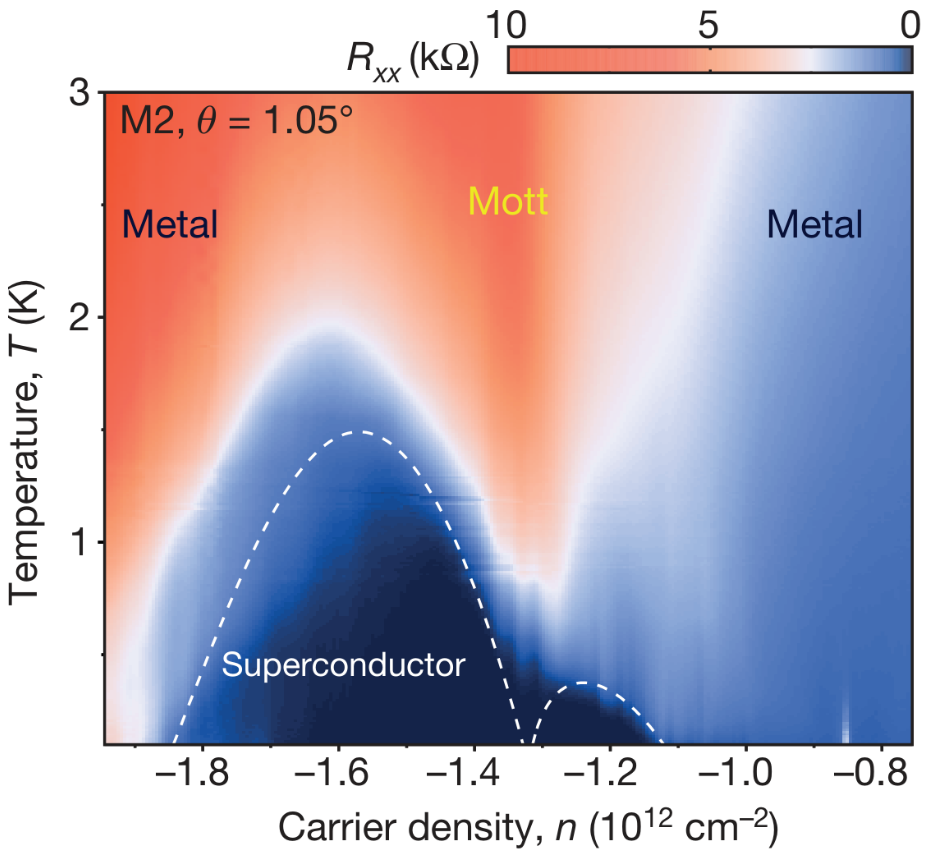
\includegraphics[height=17em]{fig/tbg_Tc_superconductivity_M2.png}
  \caption{Phase diagram for \(\theta = 1.05^\circ\) showing two asymmetric and overlapping superconducting domes with the highest critical temperature \(T_c = 1.7 \, \text{K}\).}
  \label{fig:tbg_superconductivity_b}
\end{subfigure}
\caption{Four-probe resistance \(R_{xx}\) as a function of temperature $T$ and carrier density $n$. Two superconducting domes surround the half-filling state, labeled ``Mott,'' and are centered around \(\nu = -2\) electrons per moiré unit cell. Regions outside the domes exhibit metallic behavior, characterized by a typical metallic temperature dependence. Adapted from \cite{cao2018}.}
\label{fig:tbg_superconductivity}
\end{figure}

Beyond the discovery of superconducting \cite{cao2018} and correlated insulating states \cite{cao2018_correlated}, improvements in sample quality and experimental techniques have significantly expanded the phase diagram of twisted bilayer graphene. First of all, correlated insulating states have been observed at nearly all integer fillings of the four flat bands \cite{Lu_2019, Kerelsky_2019, Choi_2019}. Notably, aligning one graphene layer with the hBN substrate reveals unexpected magnetic properties at \(\nu = 3\) fillings \cite{Serlin_2020}. In this alignment, the longitudinal resistance \(R_{xy}\) attains the quantized value \(\hbar/e^2\), accompanied by a deep minimum in \(R_{xx}\), reminiscent of an integer quantum Hall state. Moreover, the Hall resistivity exhibits hysteresis with a coercive field of several tens of millitesla, signaling the emergence of the quantum anomalous Hall effect \cite{thesis_angeli}. These findings indicate spontaneous breaking of time-reversal symmetry and suggest a non-trivial topological origin for these phenomena.

In summary, the interplay between the twist angle, electron-electron interactions, and moiré patterns in TBG gives rise to a diverse and highly tunable phase diagram, featuring superconductivity, Mott insulating states, and topological phenomena. These discoveries open new avenues for investigating exotic quantum phases in two-dimensional materials.

%%%%%%%%%%%%%%%%%%%%%%%%%%%%%%%%%%%%%%%%%%%%%%%%%%%%%%%%%%%%%%%%%%%%%%%%%%%%%%%%%%%%%%%%%%%%%%%%%%
\section{Structure of the thesis} \label{sec:outline_thesis}
%%%%%%%%%%%%%%%%%%%%%%%%%%%%%%%%%%%%%%%%%%%%%%%%%%%%%%%%%%%%%%%%%%%%%%%%%%%%%%%%%%%%%%%%%%%%%%%%%%

In this thesis, we analyze the symmetries and topology of twisted bilayer graphene (TBG), with the ultimate goal of understanding the Topological Heavy Fermion (THF) model proposed by Bernevig et al. \cite{topoheavyfermion2022}. Our work is structured as follows:

\begin{itemize}
\item Chapter \ref{ch:group_theory} introduces group theory and representation theory, providing the foundation for the following chapters. This chapter is designed to be instructional, with a focus on graphene examples, particularly the honeycomb lattice and hexagons.

\item Chapter \ref{ch:topological_quantum_chemistry} presents the Topological Quantum Chemistry (TQC) framework, which classifies topological materials based on their symmetries and band structures. This chapter builds on the group theory concepts from Chapter \ref{ch:group_theory} and sets the stage for applying TQC to TBG.

\item Chapter \ref{ch:emmergent_symm_wannier_obstruction} explores the TBG system through the Bistritzer-MacDonald model (continuum theory). Here, we analyze its geometry, emergent symmetries, and topology using TQC, and discuss the Wannier obstruction arising from the topological analysis.

\item Chapter \ref{ch:topoheavyfermion} introduces the Topological Heavy Fermion (THF) model, which maps the low-energy bands of TBG to the heavy fermion problem. The model resolves the Wannier obstruction by coupling $f$-electrons (flat bands, heavy) with $c$-electrons (nearly free), providing a comprehensive description that incorporates all emergent symmetries.

\item Finally, Chapter \ref{ch:conclusions} offers concluding remarks and reflections on the work presented.
\end{itemize}



%%%%%%%%%%%%%%%%%%%%%%%%%%%%%%%%%%%%%%%%%%%%%%%%%%%%%%%%%%%%%%%%%%%%%%%%%%%%%%%%%%%%%%%%%%%%%%%%%%
%%%%%%%%%%%%%%%%%%%%%%%%%%%%%%%%%%%%%%%%%%%%%%%%%%%%%%%%%%%%%%%%%%%%%%%%%%%%%%%%%%%%%%%%%%%%%%%%%%


%%%%%%%%%%%%%%%%%%%%%%%%%%%%%%%%% COMMENT THIS TO COMPILE main.tex %%%%%%%%%%%%%%%%%%%%%%%%%%%%%%%%
%%%-----
%%% Referências bibliográficas
%%%-----
%\addcontentsline{toc}{chapter}{\bibname}
%%\bibliographystyle{abntex2-num}
%\bibliography{citations}
%\bibliographystyle{ieeetr}
%\end{document}
%%%%%%%%%%%%%%%%%%%%%%%%%%%%%%%%% COMMENT THIS TO COMPILE main.tex %%%%%%%%%%%%%%%%%%%%%%%%%%%%%%%%
